\begin{enumerate}[label=\thesection.\arabic*.,ref=\thesection.\theenumi]
\numberwithin{equation}{enumi}
\item The number of directions and encirclements around the point -1+j0 in the complex plane by the Nyquist plot of $G(s) = \frac{1-s}{4+2s}$\\

\solution
First,we need to draw the polar plot of given G(S).
In the polar plot,substitute s = $j\omega$

\begin{align}
G(j\omega) = \frac{1-j\omega}{4+2j\omega} 
\end{align}

\begin{align}
\lim_{\omega\to\infty} G(j\omega) = \frac{1-j\omega}{4+2j\omega} 
\end{align}

\begin{align}
\lim_{\omega\to\infty} G(j\omega) = \frac{j\omega(\frac{1}{j\omega}-1)}{j\omega(\frac{4}{j\omega}+2)}  
\end{align}

\begin{align}
\lim_{\omega\to\infty} G(j\omega) = \frac{-1}{2}\angle 0  
\end{align}

\begin{center}
which is equal to $\frac{1}{2}\angle{-180}$   
\end{center}
Now substitute $\omega = 0$

\begin{align}
\lim_{\omega\to\ 0} G(j\omega) = \frac{1-j\omega}{4+2j\omega} = \frac{1}{4}\angle 0 
\end{align}

\begin{align}
\angle (G(j\omega)) = \tan^{-1}(\frac{-\omega}{1}) - \tan^{-1}(\frac{\omega}{2})
\end{align}

so from this  at $\omega = 0$ $\angle G(j\omega) = 0$ 
\\
and at $\omega = \infty$ $\angle G(j\omega)  =-180$     


\begin{align}
\mid(G(j\omega))\mid = \frac{\sqrt{1+{\omega}^2}}{\sqrt{16+{4\omega}^2}} 
\end{align}

when $\omega = 0$ $\mid(G(j\omega))\mid = \frac{1}{4}$ 
\\
and at  $\omega = \infty$ $\mid(G(j\omega))\mid = \frac{1}{2}$
\\
So,we have to plot first 0.25 on positive x-axis then we have to turn {-180} degrees from that point i.e {180} degrees clockwise(in this case).\\

Plot the Polar Plot from $\omega=0$ to $\infty$ \\
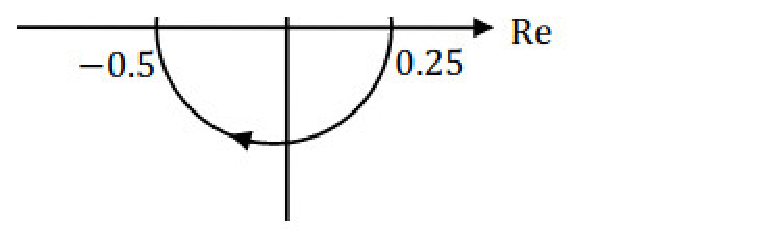
\includegraphics[width=\columnwidth]{./figs/image2.eps}\\
Draw the Mirror image of the Polar Plot.\\
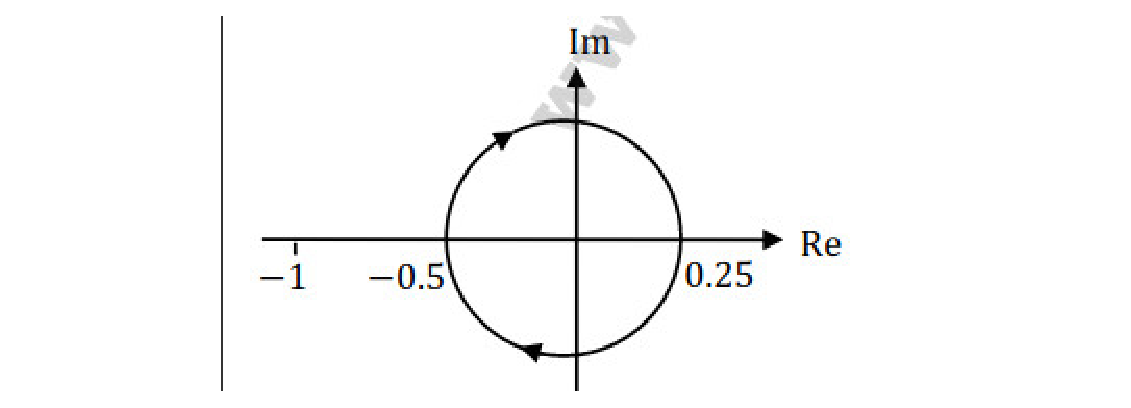
\includegraphics[width=\columnwidth]{./figs/image1.eps}\\

\begin{center}
Substitute $s = Re^{j\theta}$
\end{center}

\begin{align}
\lim_{R\to \infty}\,G(Re^{j\theta})=\frac{1-Re^{j\theta}}{4+2Re^{j\theta}}=\frac{-1}{2}  
\end{align}

As there are no $e^{j\theta}$ terms.\\
There will be no enclosed Nyquist path here.\\ 
So, for this Transfer function $G(s)$,the Nyquist plot is the the Polar plot and its mirror image with respect to real axis.\\
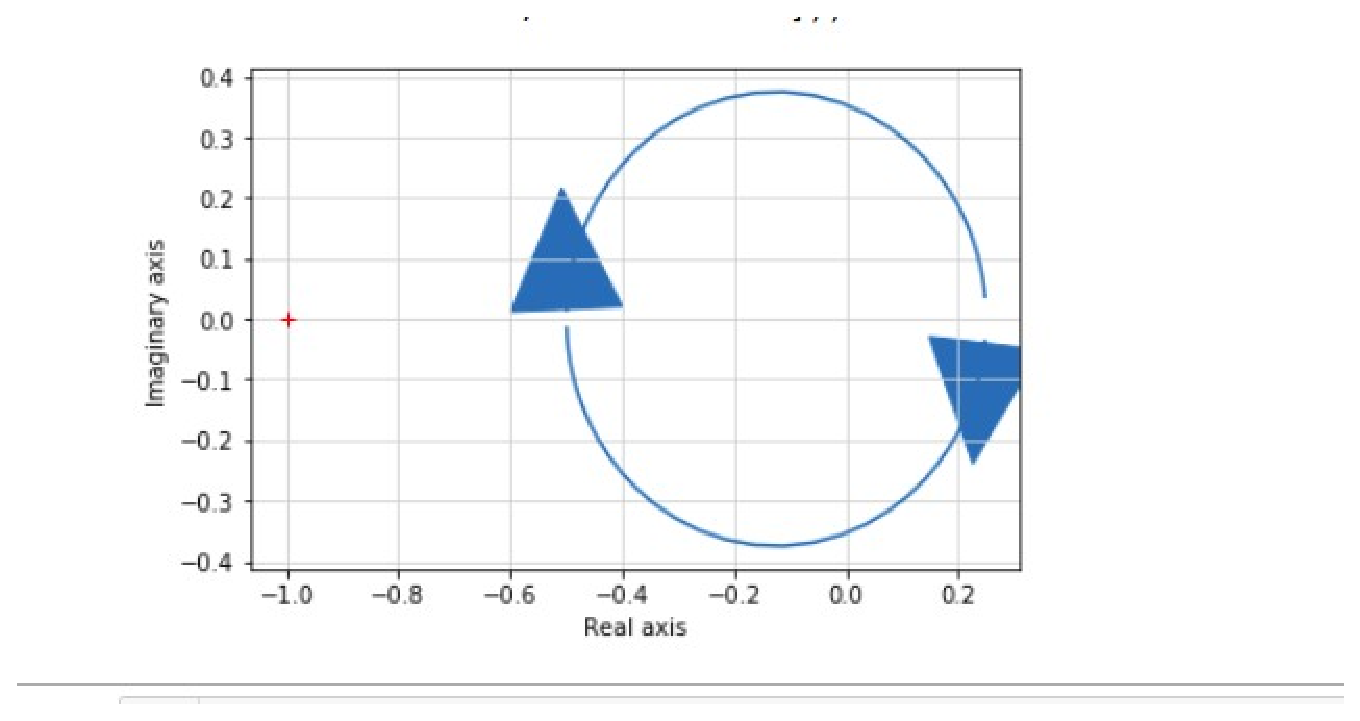
\includegraphics[width=\columnwidth]{./figs/pythonnyquistplot.eps}\\
As from the observed plot the co-ordinate -1 + j0 is outside the contour.\\
Hence,the number of encirclements around the the given co-ordinate is zero.
\end{enumerate}
